\documentclass[parskip=full]{scrartcl}
\usepackage[top=2.5cm, bottom=2.5cm, left=2.5cm, right=2.5cm]{geometry}
\usepackage[utf8]{inputenc}
\usepackage[T1]{fontenc}
\usepackage[german]{babel}
\usepackage[pangram]{blindtext}
\usepackage{hyperref}
\usepackage[toc, nonumberlist]{glossaries}
\usepackage{graphicx}
\usepackage{enumitem}
\usepackage{float}
\usepackage{color}

\hypersetup{
  colorlinks=false,
  linktoc=all,
  hidelinks,
}

%!TEX root = Pflichtenheft.tex

\newglossaryentry{Dockerimage}
{
  name=Dockerimage,
  plural=Dockerimages,
  description={Ein Container mit Programmen, der unabhängig vom zugrunde liegenden Betriebssystem gleichbleibende Bedingungen herstellt}
}

\newglossaryentry{Fertigungssimulation}
{
  name=Fertigungssimulation,
  plural=Fertigungssimulationen,
  description={Darstellung der Industrieanlage und Simulieren des Verhaltens}
}


\newglossaryentry{GUI}
{
  name=GUI,
  plural=GUIs,
  description={Die grafische Benutzerumgebung des Programms, welche vom Bediener gesehen wird}
}

\newglossaryentry{Industrial Data Space}
{
  name=Industrial Data Space,
  plural=Industrial Data Spaces,
  description={Eine Infrastruktur zum Austausch von Daten in der Industrie}
}

\newglossaryentry{Jitter}
{
  name=Jitter,
  description={Simulation von variierenden Werten, um näher an echten Anlagen zu liegen}
}

\newglossaryentry{Makro}
{
  name=Makro,
  plural=Makros,
  description={Eine aufgezeichnete Folge von Einstellungen, die gesetzt werden. Wird benutzt, um einen komplexeren Ablauf in der Anlage zu simulieren}
}

\newglossaryentry{OPC UA}
{
  name=OPC UA,
  plural=OPC UA,
  description={Ein Protokoll zur Übertragung von Daten und Steuersignalen von Industrieanlagen}
}

\newglossaryentry{Produktionsanlage}
{
  name=Produktionsanlage,
  plural=Produktionsanlagen,
  description={Großmaschinen, wie sie in der Industrie eingesetzt werden. Hier symbolisiert durch Tanks mit Flüssigkeiten}
}

\newglossaryentry{Sensordatum}
{
  name=Sensordatum,
  plural=Sensordaten,
  description={Ausgabewert eines simulierten Sensors wie Temperatur oder Durchflussmenge}
}

\newglossaryentry{Systemadapter}
{
  name=Systemadapter,
  plural=Systemadapter,
  description={Konvertiert die Daten eines Gesamtsystems (hier Industrieanlage) in ein anderes Format}
}

\newglossaryentry{TCP/IP Verbindung}
{
  name=TCP/IP Verbindung,
  plural=TCP/IP Verbindungen,
  description={Ein Protokoll zum Datenaustausch über das Internet}
}

\newglossaryentry{Uberwachungskonsole}
{
  name=Überwachungskonsole,
  plural=Überwachungskonsolen,
  description={Anzeige der Sensorwerte der Fertigungssimulation}
}

\newglossaryentry{Wrapper}
{
  name=Wrapper,
  plural=Wrapper,
  description={Programm, das ein anderes Programm umgibt und auf Ereignisse im umgebenen Programm reagieren kann}
}
\makeglossaries

\title{OSIP - Pflichtenheft}
\subtitle{\gls{OPC UA} Simulator for Industrial Plants}
\author{
    M. Armbruster\\
    D. Kahles\\
    H. Lehmann\\
    M. Schwarzmann\\
    N. Wilhelm
}

\begin{document}
\maketitle

\begin{figure}[H]
  \centering
  
\includegraphics[scale=0.5]{../icon.png}
  \caption{Icon der Anwendung}
\end{figure}
\pagebreak
\tableofcontents
\pagebreak

\section{Einleitung}
In der heutigen Zeit dringt die Vernetzung in immer neue Bereiche vor. So auch in die Industrie und ihre Fertigungsprozesse.
Dabei soll das Projekt \gls{Industrial Data Space} helfen, einen Datenraum zu erzeugen, der Datensicherheit, Datensouveränität und
Transparenz bietet. Auf diese Weise soll dazu beigetragen werden, Industrie 4.0 voranzutreiben und somit durch Vernetzung von
Maschinen, Computern und Menschen die Leistungsfähigkeit der Industrie zu erhöhen und auf die Zukunft auszurichten.
Dabei hilft das auf \gls{TCP/IP} basierende Kommunikationsprotokoll \gls{OPC UA}, Maschinen miteinander kommunizieren zu lassen.

Die hier vorgestellte Simulation (siehe Systemskizze) ermöglicht es, die Vorteile der Vernetzung von Maschinen mit \gls{OPC UA} interaktiv
zu demonstrieren, um Industriekunden von den neuen Möglichkeiten zu überzeugen. Die Hauptkomponenten sind eine \gls{Fertigungssimulation}
mit \glslink{OPC UA Server}{OPC UA Servern} und eine \gls{Uberwachungskonsole} mit \glspl{OPC UA Client}, die jeweils eine graphische
Benutzeroberfläche (\gls{GUI}) enthalten und auf getrennten Computern laufen können. Sie kommunizieren lediglich über \gls{OPC UA}.

In der GUI der \gls{Fertigungssimulation} wird eine \gls{Produktionsanlage} dargestellt.
Drei Tanks werden mit je einer farbigen Flüssigkeit gefüllt und leiten diese in einen weiteren Tank,
in dem die Flüssigkeiten durch einen Motor gemischt werden. Daten und Werte der \gls{Produktionsanlage} werden ebenfalls angezeigt. Dazu gibt
es die Möglichkeit, die Parameter der \gls{Produktionsanlage} zu konfigurieren. Dies geschieht beispielsweise indem man Zu- und Abflussmengen
einstellt. Die visuelle Darstellung passt sich an die Konfiguration an.

Die \gls{Uberwachungskonsole} liest die Daten der \gls{Fertigungssimulation}, stellt sie optisch ansprechend in einem Monitoring dar
und kann Alarme anzeigen, die vom \gls{OPC UA Server} empfangen werden. Das Monitoring ist ebenfalls konfigurierbar. Es ist etwa möglich, Filter
auf Variablen anzuwenden. Allerdings hat die \gls{Uberwachungskonsole} keinen Einfluss auf die \gls{Fertigungssimulation}.

\pagebreak
\section{Zielbestimmung}
Der \gls{Systemadapter} dient dem Ziel, die Funktion von \gls{OPC UA} zu demonstrieren, ohne eine konkrete \gls{Produktionsanlage}
benutzen zu müssen. Somit kann beim Kunden das Protokoll flexibler vorgestellt werden. Hierzu soll das Programm
sowohl eine \gls{Produktionsanlage} simulieren und deren Status graphisch darstellen, als auch auch eine \gls{Uberwachungskonsole}
bereitstellen, die über \gls{OPC UA} Werte der \gls{Produktionsanlage} abfragt.\\

\begin{figure}[H]
  \centering
  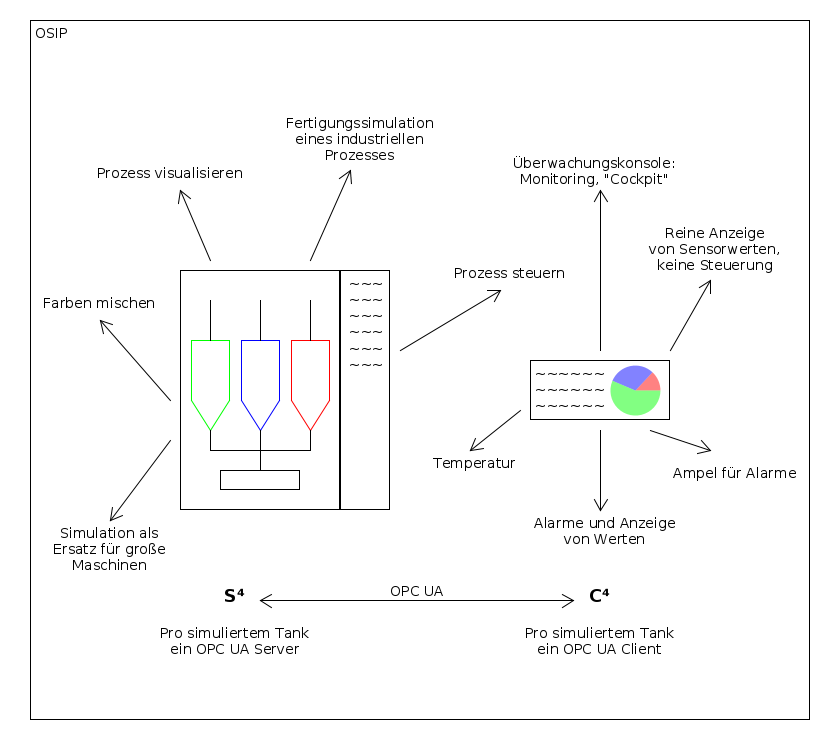
\includegraphics[scale=0.5]{../system-sketch.png}
  \caption{Systemskizze}
\end{figure}

In der Systemskizze ist links die \gls{Fertigungssimulation} bzw. stellvertretend ihre \gls{GUI} skizziert.
Darüber lässt sich das \gls{Simulations-Szenario} steuern. Die \glspl{Sensordatum} der Simulation werden 
im \gls{OPC UA Server} gesetzt, welche von einem \gls{OPC UA Client} abgefragt werden. 
Dabei stellt ein Server je einen Tank dar. Rechts davon ist die \gls{Uberwachungskonsole} eingezeichnet.
Sie zeigt die \glspl{Sensordatum} der \gls{Fertigungssimulation} mit Hilfe einer \gls{GUI} an. 
Diese Daten erhält die \gls{Uberwachungskonsole} von einem \gls{OPC UA Client}. 
Der Doppelpfeil verdeutlicht die Beziehung zwischen \glslink{OPC UA Server}{OPC UA Servern} (S) und
\glspl{OPC UA Client} (C), die den Datenaustausch unterhalb der \gls{Fertigungssimulation} und
der \gls{Uberwachungskonsole} regeln.
Dabei steht jeder \gls{OPC UA Server} mit genau einem {OPC UA Client} in Verbindung.

\subsection{Musskriterien}
\subsubsection{Allgemein}
\begin{itemize}
  \item Die verwendete \gls{Produktionsanlage} ist ein chemischer Produktionsprozess mit vier Tanks und Flüssigkeiten, die darin gemischt werden.
  \item Die Kommunikation zwischen \gls{Uberwachungskonsole} und \gls{Fertigungssimulation} findet \"uber \glspl{OPC UA Server} auf Seiten der \gls{Fertigungssimulation}
    und \glspl{OPC UA Client} auf Seiten der \gls{Uberwachungskonsole} statt.
  \item Die \gls{Fertigungssimulation} mit den \glslink{OPC UA Server}{OPC UA Servern} und die \gls{Uberwachungskonsole} mit den \glspl{OPC UA Client} laufen auf dem selben oder auf getrennten Rechnern.
\end{itemize}

\subsubsection{Überwachungskonsole}
\begin{itemize}
  \item Die \gls{Uberwachungskonsole} ruft alle \glspl{Sensordatum} der \gls{Fertigungssimulation} in einem festgelegten Zeitintervall über einen \gls{OPC UA} Client ab.
  \item Der \gls{OPC UA} Client ist mit \gls{OPC UA} Servern verbunden. Dazu ist die Einstellung der \glspl{Verbindungsinformation} möglich.
  \item Die von den \glspl{OPC UA Client} abgerufenen Werte und deren zeitlicher Verlauf werden graphisch dargestellt. Die Werte sind Zu- und Abflussmengen,
    Flüssigkeitsfarben sowie die Drehzahl eines Mischermotors.
  \item Die \gls{Uberwachungskonsole} enthält Alarme, die beim Überschreiten von Schwellenwerten in der \gls{Fertigungssimulation} durch den \gls{OPC UA} Server gesendet
    und dem Nutzer graphisch mitgeteilt werden.
\end{itemize}

\subsubsection{Fertigungssimulation}
\begin{itemize}
  \item Die \gls{Fertigungssimulation} enth\"alt eine schematische Darstellung der simulierten \gls{Produktionsanlage}.
  \item In der \gls{GUI} der \gls{Fertigungssimulation} kann der Benutzer die simulierte \gls{Produktionsanlage} steuern.
  \item Die \gls{Fertigungssimulation} aktualisiert die \glspl{Sensordatum} in den \glslink{OPC UA Server}{OPC UA Servern}.
\end{itemize}

\subsection{Kannkriterien}
\subsubsection{Allgemein}
\begin{itemize}
  \item In der \gls{Fertigungssimulation} und der \gls{Uberwachungskonsole} werden Probleme der Programmausf\"uhrung geloggt.
  \item Die Standard-Sprache Englisch kann über \glspl{Java Property Datei} in andere Sprachen übersetzt werden.
  \item Die zu verwendende Sprache ist in der \gls{GUI} einstellbar.
\end{itemize}

\subsubsection{Überwachungskonsole}
\begin{itemize}
  \item Die von den \glspl{OPC UA Client} abgerufenen Werte enthalten die Temperaturen der Flüssigkeiten in den Tanks.
  \item Das Zeitintervall für den Empfang der \glspl{Sensordatum} ist einstellbar.
  \item Die Alarme sind ein- und ausschaltbar.
  \item Die Schwellen zur Ausl\"osung der Alarme sind vom Benutzer veränderbar.
  \item Die eingestellten Alarme werden gespeichert und beim n\"achsten Programmstart automatisch wiederhergestellt.
  \item Es gibt eine Logging-Funktion.
\end{itemize}

\subsubsection{Fertigungssimulation}
\begin{itemize}
  \item Es gibt vordefinierte \glspl{Simulations-Szenario}, die über das Menü gestartet werden können.
  \item Die \glspl{Simulations-Szenario} werden in eigenen Dateien definiert. Neue \glspl{Simulations-Szenario}
    werden durch das Einf\"ugen eigener Dateien im entsprechenden Format erstellt.
  \item \gls{Jitter} in den Zuflussmengen der Tanks sorgt f\"ur Variation in den gemessenen Werten.
\end{itemize}

\subsection{Abgrenzungskriterien}
\subsubsection{Allgemein}
\begin{itemize}
  \item \gls{Fertigungssimulation} und \gls{Uberwachungskonsole} dienen der Demonstration des \glslink{OPC UA}{OPC UA Protokolls}. Dazu wird die Open Source
    Implementierung \gls{Milo} des \glslink{OPC UA}{OPC UA Protokolls} verwendet. Das \glslink{OPC UA}{OPC UA Protokoll} wird nicht selbst implementiert.
  \item Es werden verschiedene Möglichkeiten des \glslink{OPC UA}{OPC UA Protokolls} aufgezeigt, allerdings wird die kryptografische Sicherheit von \gls{OPC UA} nicht demonstriert.
\end{itemize}

\subsubsection{Überwachungskonsole}
\begin{itemize}
  \item Die \gls{Uberwachungskonsole} zeigt alle Sensorwerte und deren zeitlichen Verlauf an, stellt allerdings den Prozess nicht dar.
  \item Die \gls{Uberwachungskonsole} ist auf die \gls{Fertigungssimulation} abgestimmt. Es sollen damit nicht beliebige
    Fertigungsprozesse \"uberwacht werden k\"onnen.
  \item Die \gls{Uberwachungskonsole} dient ausschlie{\ss}lich der \"Uberwachung der Daten, die von der \gls{Fertigungssimulation}
    stammen. Sie kann nicht steuernd in die \gls{Fertigungssimulation} eingreifen.
\end{itemize}

\subsubsection{Fertigungssimulation}
\begin{itemize}
  \item Die \gls{Fertigungssimulation} stellt eine einzelne \gls{Produktionsanlage} schematisch dar. Die Darstellung verschiedener \glspl{Produktionsanlage}
    ist nicht das Ziel. Eine realistisch-detaillierte Simulation ist nicht das Ziel.
\end{itemize}


\newpage
\section{Produkteinsatz}
\subsection{Anwendungsbereiche}
Das Produkt wird verwendet, um \gls{OPC UA} und dessen Möglichkeiten zu präsentieren.
Insbesondere soll es einfacher aufzubauen und zu zeigen sein als reale \glspl{Fertigungssimulation}.
Dies kann zum Beispiel auf Messen oder direkt bei potenziellen Kunden geschehen.

\subsection{Zielgruppen}
Die Zielgruppe umfasst Personen, die sich mit \gls{OPC UA} auskennen und es potenziellen Anwendern vorführen möchten.
Dazu zählen insbesondere Mitglieder der OPC Foundation, die die Verbreitung des Protokolls fördern wollen, und Personen, die im \gls{Industrial Data Space} beschäftigt sind,
aber auch Softwareentwickler, die \gls{OPC UA} konforme Software herstellen und möglichen Kunden auf einfache Art und
Weise die Funktionalität von \gls{OPC UA} präsentieren wollen.
Die potenziellen Anwender haben meist keine Erfahrung mit \gls{OPC UA}, sind aber für \glspl{Produktionsanlage} verantwortlich,
die von \gls{OPC UA} profitieren würden.

\subsection{Betriebsbedingungen}
Das Produkt kann entweder auf Messen, in Büros oder in Fertigungshallen direkt bei Kunden verwendet werden,
so lange die eingesetzte Hardware (siehe \ref{Hardware}) keine Probleme mit den Umgebungsbedingungen hat.

\pagebreak
\section{Produktumgebung}
\subsection{Software}
Das Produkt erfordert einen Computer, auf dem das Betriebssystem Microsoft Windows 10, Canonical Ubuntu 16.04 oder Linux Mint 18 installiert ist,
Außerdem ist das Oracle Java Runtime Environment in Version 1.8
notwendig. Wenn die \gls{Fertigungssimulation} und die \gls{Uberwachungskonsole} auf unterschiedlichen Computern laufen,
ist eine \gls{TCP/IP} Verbindung mit einer Bandbreite von 100 MBit/s und einer Latenz von maximal 100 ms zwischen den Computern notwendig.
Außerdem wird eventuell (siehe \ref{fertigung-optional} und \ref{konsole-optional}) unter Ubuntu 16.04 die Containersoftware Docker
ab Version 1.10.3 unterstützt, mit dem die beiden Softwareteile isoliert in Containern verteilt und ausgeführt werden können.

\subsection{Hardware}
\label{Hardware}
Es ist ein Laptop oder Desktopcomputer notwendig, der eines der oben genannten Betriebssysteme unterstützt.
Zudem sind mindestens 2GB Arbeitsspeicher notwendig. Die CPU muss die x86 Architektur unterstützen, zwei Kerne haben und mit
mindestens 2GHz getaktet sein.

\pagebreak
\section{Funktionale Anforderungen}
Im Nachfolgenden sind die Nummern optionaler Funktionalitäten, die sich aus den Kann-Kriterien ergeben, \textcolor{blue}{blau} markiert.

\subsection{Fertigungssimulation}
\subsubsection{Funktionalität}
\begin{enumerate}	
  \item[FA10] Es gibt eine .jar Datei, die bei Ausführung die \gls{Fertigungssimulation} sowie zugehörige \glspl{OPC UA Server} startet.
  \item[\textcolor{blue}{FA20}] Es gibt ein \gls{Dockerimage} zur einfachen Verteilung und isolierten Ausführung der \gls{Fertigungssimulation}.  
  \item[FA30] Die \gls{Fertigungssimulation} wird nach der Model-View-Controller-Architektur entworfen.
  \item[FA40] Der Betrieb der \gls{Produktionsanlage} wird simuliert und grafisch dargestellt.
  \item[FA50] Die \gls{Produktionsanlage} wird innerhalb der \glspl{OPC UA Server} repräsentiert.
  \item[FA60] Die Ports, über welche die einzelnen \gls{OPC UA Server} der \gls{Fertigungssimulation} kommunizieren, können eingestellt werden.
  \item[FA70] Die \gls{Fertigungssimulation} aktualisiert die \glspl{Sensordatum} ihrer \glspl{OPC UA Server}.    
  \item[FA80] Die \glspl{OPC UA Client} der \gls{Uberwachungskonsole} registrieren sich bei den \glslink{OPC UA Server}{OPC UA Servern} der \gls{Fertigungssimulation} und empfangen von
    diesen \glspl{Sensordatum}.
  \item[FA90] Nach Anforderung durch die \gls{Uberwachungskonsole} wird in bestimmten, der Anfrage definierten Zust\"anden ein Alarm an die \glspl{OPC UA Client} der \gls{Uberwachungskonsole} gesendet.
  \item[\textcolor{blue}{FA100}] Fehler und Ausnahmen bei der Ausführung werden geloggt.  
  \item[\textcolor{blue}{FA110}] Die \gls{Fertigungssimulation} verfügt über einen \gls{Jitter}.
  \item[\textcolor{blue}{FA120}] Die \gls{Fertigungssimulation} besitzt vordefinierte \glspl{Simulations-Szenario}, die über das Menü gestartet werden können. Somit kann ohne aktive Nutzerinteraktion eine sich
    im aktiven Betrieb befindliche \gls{Produktionsanlage} simuliert werden.
\end{enumerate}

\subsubsection{GUI Darstellung}
\begin{enumerate}
  \item[FA130] Die \gls{GUI} der \gls{Fertigungssimulation} zeigt drei Flüssigkeitstanks, die auf einer Höhe sind, und einen weiteren Flüssigkeitstank unter den oberen drei.
    Es führen Leitungen von den drei oberen Tanks zum unteren Tank.
  \item[FA140] An jeder Leitung befinden sich ein Ventil sowie ein Durchflussmesser in Form eines sich drehenden Elements. Der Öffnungsgrad des Ventils wird prozentual auf dem Ventil angezeigt.
  \item[FA150] Die Zu- und Abflussmengen der oberen (siehe FA110) Flüssigkeitstanks können separat eingestellt werden.
  \item[FA160] Die Abflussmenge des unteren (siehe FA110) Flüssigkeitstanks kann eingestellt werden. Die Zuflussmenge ergibt sich aus der Summe der Abflussmengen der oberen Tanks.
  \item[FA170] Jedem der oberen Tanks ist eine feste Flüssigkeitsfarbe zugeordnet. Die Farbe des unteren Tanks ergibt sich aus dem Mischungsverhältnis der oberen Tanks. Dabei wird
	angenommen, dass die Flüssigkeiten der oberen Tanks die selbe Deckkraft haben.
  \item[FA180] Der linke obere Tank wird mit roter, der mittlere mit grüner und der rechte mit blauer Flüssigkeit gefüllt.
  \item[FA190] Die Füllstände der Tanks werden gemessen.
  \item[FA200] Der Füllstand der Flüssigkeitstanks wird durch das Füllen der Tanks in der Farbe ihrer Flüssigkeit dargestellt.
  \item[FA210] Der untere Tank enthält einen motorbetriebenen Mischer, dessen Drehzahl eingestellt werden kann.
  \item[FA220] Der Mischer im unteren Tank wird durch ein sich drehendes \gls{GUI} Element dargestellt.
    Die Umdrehungsgeschwindigkeit repräsentiert die Drehzahl des Mischermotors.
  \item[\textcolor{blue}{FA230}] An jedem Tank ist ein Temperatursensor angebracht.
  \item[\textcolor{blue}{FA240}] Die Zuflusstemperaturen der oberen Tanks können separat eingestellt werden.
  \item[FA250] Jeder der dargestellten Tanks ist mit einer hellgrauen Box hinterlegt, welche den Zuständigkeitsbereich des jeweiligen \glslink{OPC UA Server}{OPC UA Servers} repräsentiert.
  \item[FA260] Kommt es in der \gls{Fertigungssimulation} zu einem \"Uberlauf, so h\"alt die \gls{Fertigungssimulation} an und es wird der Text "`\"Uberlauf"' angezeigt.
  \item[FA270] Das System wird aus einem "`\"Uberlauf"' durch den Knopf "`Zur\"ucksetzen"' im gezeigten Dialog wieder in den Startzustand versetzt. Anschlie{\ss}end wird die Ausführung fortgesetzt.	
  \item[FA280] Die \gls{Fertigungssimulation} besitzt einen "`Über"'-Dialog, welcher Lizenzinformationen zu verwendeten Bibliotheken
    sowie eine kurze Information zu den Erstellern des Programms, enthält.
  \item[FA290] Der Menüeintrag "`Szenarien"' zeigt eine Liste der \glspl{Simulations-Szenario}, die durch einen Klick gestartet werden können.
  \item[FA300] Die einstellbaren Parameter können in einem Einstellungsdialog festgelegt werden. Darin existiert für jeden Tank ein eigener Reiter, der die 
    tankspezifischen Einstellungen, wie zum Beispiel Zu- und Abflussmengen, Zuflusstemperaturen oder Motordrehzahlen enthält.
    Diese Parameter werden durch Schieberegler eingestellt.
  \item[\textcolor{blue}{FA310}] Der Einstellungsdialog besitzt einen Regler, welcher den \gls{Jitter} konfigurierbar macht.
    Hierbei entspricht ein \gls{Jitter} von 0 der Deaktivierung der Funktion.
  \item[\textcolor{blue}{FA320}] Im Einstellungsdialog kann die Sprache der \gls{Fertigungssimulation} bestimmt werden.
  \item[FA330] Die Standardsprache der \gls{GUI} ist Englisch.
  \item[FA340] Der Einstellungsdialog besitzt Knöpfe zum Verwerfen ("`Abbrechen"') und Anwenden ("`Speichern"') der Änderungen. Ein Klick auf einer der beiden Knöpfe schließt zudem den Dialog.    
\end{enumerate}

\subsection{Überwachungskonsole}
\subsubsection{Funktionalität}
\begin{enumerate}
  \item[FA350] Es gibt eine .jar-Datei, die bei Ausführung die \gls{Uberwachungskonsole} startet.
  \item[\textcolor{blue}{FA360}] Es gibt ein \gls{Dockerimage} zur einfachen Verteilung und isolierten Ausführung der \gls{Uberwachungskonsole}.
  \item[FA370] Die \gls{Uberwachungskonsole} wird nach der Model-View-Controller-Architektur entworfen.
  \item[FA380] Die \gls{Uberwachungskonsole} enthält vier \glspl{OPC UA Client}, von denen sich jeder mit einem \gls{OPC UA Server} der \gls{Fertigungssimulation} verbindet und mit diesem über \gls{TCP/IP} per
    \gls{OPC  UA} kommuniziert.
  \item[FA390] Die \glspl{OPC UA Client} erhalten die \glslink{TCP/IP}{IP-Adresse}, die durch die \gls{Uberwachungskonsole} nicht geändert werden kann, des verwendeten Computers.
  \item[FA400] Die \glspl{OPC UA Client} erhalten beim Start die Ports automatisch durch das Betriebssystem.
  \item[FA410] Beim Start versucht die \gls{Uberwachungskonsole}, eine Verbindung zwischen den \glspl{OPC UA Client} und den \glslink{OPC UA Server}{OPC UA Servern} herzustellen und sich so bei der
    \gls{Fertigungssimulation} zu registrieren.
  \item[FA420] Alle angezeigten \glspl{Sensordatum} werden mit einer festen Frequenz aktualisiert. Dabei fragen die \glspl{OPC UA Client} die Daten der \glspl{OPC UA Server}
    ab und stellen sie anschlie{\ss}end der \gls{Uberwachungskonsole} bereit.
  \item[FA430] Alarme mit ihrem jeweiligen Auslöser werden bei den \glslink{OPC UA Server}{OPC UA Servern} der \gls{Fertigungssimulation} registriert. Sie werden von den
    \glslink{OPC UA Client}{OPC UA Clients} der \gls{Uberwachungskonsole} empfangen und an die \gls{Uberwachungskonsole} weitergeleitet.
  \item[FA440] Alarme werden asynchron zu den \glspl{Sensordatum} empfangen.
  \item[\textcolor{blue}{FA450}] Bereits registrierte Alarme können wieder gelöscht werden.    
  \item[\textcolor{blue}{FA460}] Geloggt werden Fehler und Ausnahmen während der Ausführung der \gls{Uberwachungskonsole} sowie alle eintreffenden Alarme.
\end{enumerate}

\subsubsection{GUI Darstellung}
\begin{enumerate}
  \item[FA470] Die \gls{Uberwachungskonsole} stellt die \glspl{Sensordatum} und Alarme jedes Flüssigkeitsanks in einem eigenen Bereich dar.
  \item[FA480] Die \gls{Uberwachungskonsole} zeigt die Farbe der Tanks an.
  \item[FA490] Die \gls{Uberwachungskonsole} zeigt die Zuflussmenge der oberen Tanks auf jeweils einer Skala an.
  \item[FA500] Die \gls{Uberwachungskonsole} zeigt die Abflussmenge aller Tanks auf jeweils einer Skala an.
  \item[FA510] Die \gls{Uberwachungskonsole} zeigt den Füllstand aller Tanks auf jeweils einer Skala an.
  \item[\textcolor{blue}{FA520}] Die \gls{Uberwachungskonsole} zeigt die Temperatur aller Tanks auf jeweils einer Skala an.
  \item[FA530] Die \gls{Uberwachungskonsole} zeigt die Drehzahl des Mischermotors im unteren Tank auf einer Skala an.
  \item[FA540] Der zeitliche Verlauf des Füllstandes wird jeweils für alle Tanks angezeigt.
  \item[FA550] Der zeitliche Verlauf der Temperatur wird jeweils für alle Tanks angezeigt.
  \item[FA560] Die \gls{Uberwachungskonsole} registriert für jeden Tank jeweils einen Alarm für einen Überlauf.
  \item[FA570] Die \gls{Uberwachungskonsole} registriert für jeden Tank jeweils einen Alarm für einen Unterlauf.
  \item[FA580] Ein Alarm wird durch einen Bezeichner und einen Kreis als Zustandssymbol dargestellt.
  \item[FA590] Ist der Kreis rot, wurde der Alarm ausgelöst.
  \item[FA600] Ist der Kreis grün, ist der Alarm nicht ausgelöst.
  \item[\textcolor{blue}{FA610}] Der Benutzer kann die Schwellenwerte der Alarme direkt an der Anzeige [FA580] ändern.
  \item[FA620] Der Benutzer wird über einen Dialog und durch einen roten Kreis der Anzeige des entsprechenden Alarms direkt benachrichtigt, sobald sie ausgelöst werden.
  \item[FA630] Ein Alarm wird als ausgelöst angezeigt, womit dessen Kreis rot ist, nachdem die \gls{Uberwachungskonsole} durch die \gls{Fertigungssimulation} darüber benachrichtigt wurde und bis der Alarm in der
    \gls{Fertigungssimulation} nicht mehr aktiv ist und die \gls{Uberwachungskonsole} mit der nächsten Aktualisierung der \glspl{Sensordatum} über das Ende informiert wurde.
  \item[FA640] Es gibt eine zweistufige Ampel für den allgemeinen Zustand der \gls{Uberwachungskonsole}.
  \item[FA650] Ist die Ampel rot, wurde mindestens ein Alarm ausgelöst.
  \item[FA660] Ist die Ampel grün, wurde kein Alarm ausgelöst.
  \item[\textcolor{blue}{FA670}] Es gibt eine Loggingkonsole in Form einer mehrzeiligen Textausgabe, die die geloggten Ereignisse der \gls{Uberwachungskonsole} ausgibt.
  \item[FA680] Der Menüeintrag "`Über'" öffnet ein neues Fenster, in dem der Programmname, die Version, das Programmsymbol und die Lizenz einschließlich der Lizenzen verwendeter Bibliotheken angezeigt werden.
  \item[FA690] Der Menüeintrag "`Einstellungen"' öffnet ein separates Fenster.
  \item[FA700] In den Einstellungen werden die \glslink{TCP/IP}{IP-Adresse} der \glslink{OPC UA Client}{OPC UA Clients} und der \gls{OPC UA Server} sowie deren Ports angezeigt.
  \item[FA710] In den Einstellungen sind die Ports und die IP-Adresse der \glspl{OPC UA Server} konfigurierbar.
  \item[\textcolor{blue}{FA720}] In den Einstellungen sind die Ports der \glspl{OPC UA Client} konfigurierbar.
  \item[FA730] Leere Eingaben für die Ports der \glspl{OPC UA Client} bedeuten, dass diese nicht festgelegt wurden und automatisch durch das Betriebssystem bezogen werden.
  \item[\textcolor{blue}{FA740}] In den Einstellungen ist es dem Nutzer möglich, die Sprache auszuwählen.
  \item[FA750] Die Standardsprache ist Englisch.
  \item[\textcolor{blue}{FA760}] Der Nutzer kann das Zeitintervall für die Aktualisierung der Werte über einen Schieberegler oder eine Textbox einstellen.
  \item[\textcolor{blue}{FA770}] Die Aufnahme des zeitlichen Verlaufs jedes Füllstandes und jeder Temperatur ist ein- und ausschaltbar.
  \item[\textcolor{blue}{FA780}] Der Nutzer kann die verfügbaren Alarme ein- und ausschalten und deren Schwellenwerte festlegen.
  \item[FA790] Die Eingaben in den Einstellungen werden direkt nach Eingabe auf richtige Formatierung und Einhaltung des Wertebereichs gepr\"uft.
  \item[FA800] Der Benutzer wird über eine Fehleingabe und deren Ursache informiert.
  \item[FA810] Nach Drücken eines Abbruch-Knopfes im Einstellungsfenster bleiben die Einstellungen unverändert.
  \item[FA820] Nach Drücken eines Speichern-Knopfes im Einstellungsfenster werden alle vorhandenen Einstellungen mit denen aus dem Fenster überschrieben.
  \item[FA830] Werden Einstellungen für die \glspl{OPC UA Server} oder \glspl{OPC UA Client} überschrieben, werden die \glspl{OPC UA Client} mit den neuen Einstellungen neu gestartet.
  \item[FA840] Schlägt die Verbindung zischen den \glspl{OPC UA Client} und \glslink{OPC UA Server}{OPC UA Servern} fehl oder verliert mindestens ein \gls{OPC UA Client} die Verbindung zu seinem \gls{OPC UA Server}, wird 
    der Benutzer über einen Dialog informiert und das Einstellungsfenster zur Eingabe der \gls{IP-Adresse} und Ports der \glspl{OPC UA Server} öffnet sich.
\end{enumerate}

\pagebreak
\section{Nichtfunktionale Anforderungen}
\subsection{Fertigungssimulation}
\begin{enumerate}
  \item[NF] Standardmäßig haben die \glspl{OPC UA Server} die Ports 8080, 8081, 8082 und 8083.
  \item[NF10] Die Drehzahl des Mischermotors kann vom Benutzer in einem Bereich zwischen 0 und 300 Umdrehungen pro Minute gewählt werden.
  \item[NF] Standardmäßig hat der Mischermotor 250 Umdrehungen pro Minute.
  \item[NF20] Wenn Parameter verändert werden, sind sie nach spätestens einer halben Sekunde per \gls{OPC UA} abrufbar.
  \item[NF30] Wenn der Zufluss eines Tanks komplett geschlossen, und der Ablauf komplett geöffnet wird, ist der Tank in etwa 10 Sekunden leergelaufen.
  \item[NF40] Wenn der Zufluss eines Tanks komplett geöffnet, und der Ablauf komplett geschlossen wird, ist der Tank in etwa 10 Sekunden übergelaufen.
\end{enumerate}

\subsection{Überwachungskonsole}
\begin{enumerate}
  \item[NF110] IP-Adressen müssen gültige IPv4 Adressen oder Hostnamen sein. % Abkürzungsverzeichnis für Dinge wie IPv4?
  \item[NF120] Ports dürfen Werte im Bereich 1024 bis 61000 annehmen.
  \item[NF130] Die Schwellenwerte für die Alarme dürfen zwischen 0 und 100 \% gewählt werden.
  \item[NF] Standardmäßig liegt der Schwellenwert für einen Unterlauf bei 5 \%.
  \item[NF] Standardmäßig liegt der Schwellenwert für einen Überlauf bei 95 \%.
  \item[NF140] Die Aktualisierungsfrequenz kann vom Benutzer im Bereich zwischen 100 und 4000 Millisekunden (ms) gewählt werden.
  \item[NF] Standardmäßig liegt die Aktualisierungsfrequenz bei 1000 ms.
  \item[NF150] Wenn sich Werte in der \gls{Fertigungssimulation} ändern, werden die Änderungen spätestens nach der Zeitspanne von
    einer halben Sekunde plus dem Aktualisierungsintervall in der \gls{Uberwachungskonsole} angezeigt.
\end{enumerate}

\pagebreak
\section{Produktdaten}
\begin{enumerate}
  \item[D10] Die \gls{Uberwachungskonsole} speichert die zuletzt eingestellten Ports der \glslink{OPC UA Client}{OPC UA Clients} (sofern implementiert).
  \item[D20] Die \gls{Uberwachungskonsole} speichert die zuletzt eingestellte IP-Adresse und Ports der \gls{OPC UA Server} (sofern implementiert).
  \item[D30] Die \gls{Uberwachungskonsole} speichert die zuletzt eingestellte Aktualisierungsfrequenz für die \glspl{Sensordatum} (sofern implementiert).
  \item[D40] Die \gls{Uberwachungskonsole} speichert die zuletzt eingeschalteten Alarme und alle Schwellenwerte (sofern implementiert).
  \item[D50] Die \gls{Uberwachungskonsole} speichert, welche Verläufe zuletzt angezeigt wurden (sofern implementiert).
  \item[D60] Die \gls{Uberwachungskonsole} speichert empfangene Alarme in einer Log-Datei (sofern implementiert).
  \item[D70] Die \gls{Uberwachungskonsole} speichert Fehler und Ausnahmen bei der Ausführung in einer Log-Datei (sofern implementiert).
  \item[D110] Die \gls{Fertigungssimulation} speichert die zuletzt genutzten Ports der \glspl{OPC UA Server} (sofern implementiert).
  \item[D120] Die \gls{Fertigungssimulation} speichert den zuletzt eingestellten \gls{Jitter} (sofern implementiert).
  \item[D130] Die \gls{Fertigungssimulation} speichert \glspl{Simulations-Szenario} in einzelnen Dateien (sofern implementiert).
  \item[D140] Die \gls{Fertigungssimulation} speichert Fehler und Ausnahmen bei der Ausführung in einer Log-Datei (sofern implementiert).
\end{enumerate}

\pagebreak
\section{Globale Testfälle}
\Blindtext[1]

\pagebreak
\section{Systemmodelle}
\subsection{Szenarien}
\subsubsection*{Akteure}
\textbf{Manuel}: Der Benutzer des Programms, der \gls{OPC UA} vermarkten will.\\
\textbf{Philipp}: Ein potenzieller Anwender von \gls{OPC UA}, der das Protokoll noch nicht kennt.

\subsubsection{Szenario 1: Unabhängige Installation}
Manuel möchte Philipp, einem Kunden aus der Industrie, zeigen, was mit modernen Industrie 4.0 Techniken möglich ist.
Da Philipp nur wenig Zeit hat, fährt Manuel mit dem Auto zu Philipp. Weil Manuel weder Platz noch Zeit für das
Mitführen einer kompletten Demonstrationsanlage hat, nimmt er einen Laptop mit Simulationssoftware mit.

Vor Ort angekommen startet er auf dem Laptop zwei virtuelle Maschinen, auf denen je ein Programm installiert ist.
Auf der einen virtuellen Maschine eine \gls{Fertigungssimulation} und auf der anderen virtuellen Maschine
eine \gls{Uberwachungskonsole}, um die simulierte Fertigung zu überwachen.
Nun weist Manuel den beiden virtuellen Maschinen je eine feste IP-Adresse zu.
Anschlie{\ss}end startet Manuel erst die \gls{Fertigungssimulation} und dann die \gls{Uberwachungskonsole}.
Beim Start der \gls{Uberwachungskonsole} wird er nach IP-Adresse und Ports gefragt, unter denen die \gls{Fertigungssimulation} zu finden ist.
Er gibt die Adresse der anderen virtuellen Maschine an, belässt die Ports auf dem Standard-Wert
und auch die \gls{Uberwachungskonsole} startet erfolgreich.
Nun ist klar, dass die beiden Programme tatsächlich ausschließlich über das Netzwerk kommunizieren.

In der \gls{Fertigungssimulation} wird nach dem Starten eine \gls{Produktionsanlage} angezeigt, in der Flüssigkeiten aus drei Tanks
in einem weiteren Tank vermischt werden; Farben des Inhalts der Ursprungs- und des Zieltanks visualisieren den Vorgang. 
Im Zieltank dreht sich ein Motor, der für die Durchmischung sorgt.
Es gibt Sensoren für Temperatur, Farbe, Füllstand und Durchfluss der Tanks sowie für die Drehzahl des Motors.
In der \gls{Uberwachungskonsole} sieht Philipp nun eine Reihe von Anzeigen, die sich automatisch aktualisieren und
die Zu- und Abfluss, Farbe und Temperatur der verschiedenen Tanks zeigen.

\subsubsection{Szenario 2: Konfigurierbarkeit}
Als Philipp zu ihm kommt, will Manuel ihm die Funktion von \gls{OPC UA} demonstrieren.
Als erstes ändert er in der \gls{Fertigungssimulation} den Zu- und Abfluss bei zwei der Tanks. Nun sehen die beiden, wie
sich die von der \gls{Uberwachungskonsole} angezeigten Werte für Zu- und Abfluss mit der nächsten Aktualisierung ändern. Die
Farbe im Zieltank ändert sich langsam, während sich das Mischungsverhältnis der Flüssigkeiten ändert. Auch diese
Werte werden in der \gls{Uberwachungskonsole} jeweils aktualisiert.

Als nächstes betrachten die beiden, wie sich in der \gls{Uberwachungskonsole} die Anzeigen für den Füllstand der Tanks ändern.
Außerdem verweist Manuel auf Reiter unterhalb der Überwachungsanzeigen der Tanks,
in denen Philipp die Füllstands- und Temperaturverläufe ansehen kann.

Philipp merkt nun an, dass ihm die Flexibilität der empfangenen Daten sehr gefällt. Das Aktualisierungsintervall von
einer Sekunde sei aber in seinen konkreten Fertigungsprozessen zu lang, da in kritischen Zuständen sehr schnell
reagiert werden muss, etwa wenn Schwellenwerte überschritten werden. Daraufhin ändert Manuel in den
Einstellungen das Aktualisierungsintervall von 1000ms auf 250ms. Anschließend sehen beide, wie sich die Werte in der
\gls{Uberwachungskonsole} tatsächlich vier Mal pro Sekunde aktualisieren.

\subsubsection{Szenario 3: Alarme}
Philipp ist zunehmend an \gls{OPC UA} interessiert, hat aber noch letzte Zweifel. Er merkt an, dass die Abfrage der Daten
zwar gut funktioniert, eine wirkliche \"Uberwachung aber noch eine Funktion ben\"otigen w\"urde,
um ungew\"ohnliche Zust\"ande in der Fertigung automatisch zu erkennen und darauf aufmerksam zu machen.
Manuel merkt an, dass das ein guter Einwand ist und dass \gls{OPC UA} auch daf\"ur eine passende Funktionalit\"at besitzt.

Er \"offnet das Einstellungsmen\"u der \gls{Uberwachungskonsole} und ruft den Reiter "`Alarme"' auf. Um die Flexibilit\"at
von \gls{OPC UA} erneut zu demonstrieren, fragt er Philipp, welchen vorhandenen Zustand er gerne abfangen w\"urde. Philipp möchte gerne
wissen, wenn ein Tank \"uberzulaufen droht. Er schl\"agt daf\"ur als Grenze einen F\"ullstand von 95\% vor.
Manuel aktiviert also den Alarm für Überlauf des roten Tanks und trägt als Schwelle 95\% ein.
Dann speichert er die neuen Einstellungen.

Anschlie{\ss}end startet er in der \gls{Fertigungssimulation} ein vordefiniertes Simulations-Szenario für einen Überlauf
des roten Tanks, woraufhin der F\"ullstand zu steigen beginnt. In der \gls{Uberwachungskonsole} werden ebenfalls steigende Werte angezeigt.
Darauf wird der F\"ullstand von 95\% erreicht und in der \gls{Uberwachungskonsole} ein entsprechender Dialog angezeigt. Manuel
beschlie{\ss}t, nicht zu handeln. Die \gls{Fertigungssimulation} meldet das Überlaufen eines Tanks.
Danach w\"ahlt Philipp in der \gls{Fertigungssimulation} die Option "`zur\"ucksetzen"',
woraufhin wieder die Standardkonfiguration angezeigt wird.

\subsection{Anwendungsfälle}
\subsubsection{Anwendungsfalldiagramme}
\begin{figure}[H]
  \centering
  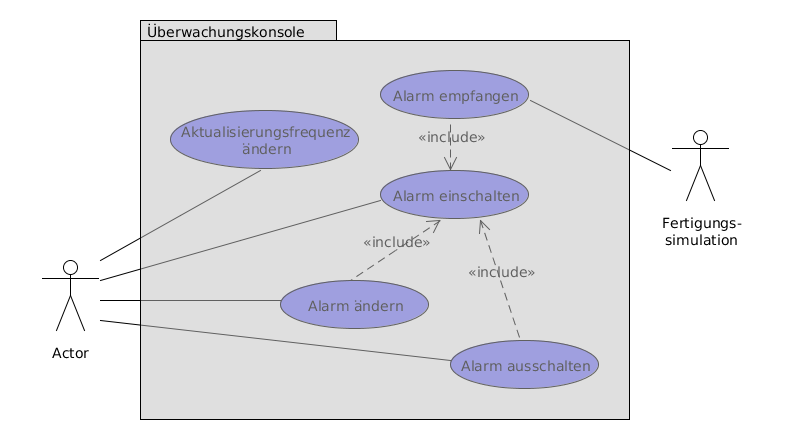
\includegraphics[scale=0.62]{media/UseCases/Ueberwachungskonsole.png}
  \caption{Anwendungsfalldiagramm für die Überwachungskonsole}
\end{figure}
\begin{figure}[H]
  \centering
  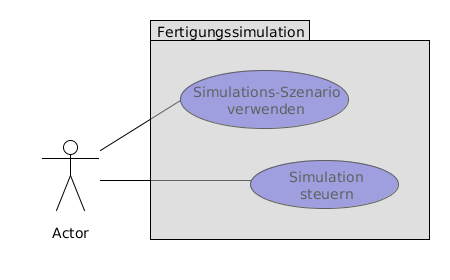
\includegraphics[scale=0.62]{media/UseCases/Fertigungssimulation.png}
  \caption{Anwendungsfalldiagramm für die Fertigungssimulation}
\end{figure}

\subsubsection{Änderung der Prozessvariablen}
\begin{description}
  \item[Name] Anpassen der Variablen wie Zu- oder Abflussgeschwindigkeit, Temperatur oder Motordrehzahl bei einem der
  Flüssigkeitstanks, sofern er die Anpassung dieser Werte erlaubt.
  \item[Akteure] Manuel (Bediener der Software)
  \item[Eingangsbedingung] Die \gls{Fertigungssimulation} und die \gls{Uberwachungskonsole} sind in Betrieb und miteinander verbunden.
  \item[Ereignisfluss]~\\
\begin{itemize}[noitemsep]
  \item Manuel öffnet das Steuerungsfenster.
  \item Manuel wählt den Reiter des Tanks, den er verändern will.
  \item Manuel stellt den gewünschten Wert ein.
  \item Manuel klickt den "`OK"' Knopf.
\end{itemize}
  \item[Ausgangssituation] Die Prozessvariable ist geändert. Dies ist in der GUI der Fertigungssimulation sichtbar, etwa durch schnelleres Befüllen oder Leeren eines Tanks,
  durch ein schnelleres Drehen der Motorvisualisierung oder durch eine Statusanzeige.
    Außerdem zeigt die \gls{Uberwachungskonsole} die geänderte Variable an.
  \item [Nichtfunktionale Anforderungen] Die geänderte Variable wird mit der nächsten Aktualisierung auf der \gls{Uberwachungskonsole} angezeigt.
\end{description}

\subsubsection{Änderung der Verbindungseinstellungen}
\begin{description}
  \item[Name] Verändern der Verbindungseinstellungen.
  \item[Akteure] Manuel (Bediener der Software)
  \item[Eingangsbedingung] Die \gls{Fertigungssimulation} und die \gls{Uberwachungskonsole} sind in Betrieb und miteinander verbunden.
  \item[Ereignisfluss]~\\
  \begin{itemize}[noitemsep]
    \item Manuel öffnet in der \gls{Uberwachungskonsole} die allgemeinen Einstellungen.
    \item Manuel stellt die Aktualisierungsfrequenz, die \gls{IP-Adresse} oder einen Port der \gls{OPC UA Server} ein.
    \item Manuel klickt den "`Speichern"' Knopf und das Einstellungsfenster schließt sich.
    \item Der Verbindungsaufbau schlägt fehlt und das Einstellungsfenster öffnet sich wieder.
    \item Manuel trägt nun die richtigen Ports und \gls{IP-Adresse} ein und klickt den "`Speichern"' Knopf.
  \end{itemize}
  \item[Ausgangssituation] Die \glspl{Sensordatum} in der \gls{Uberwachungskonsole} werden nun in Abständen der gewählten Aktualisierungsfrequenz aktualisiert.
  Wenn sich die \gls{IP-Adresse} oder Ports verändert haben, verbinden sich die betroffenen \glspl{OPC UA Client} neu mit dem Server.
  \item [Nichtfunktionale Anforderungen] Die Frequenz ändert sich spätestens mit der nächsten Aktualisierung.
\end{description}

\subsubsection{Erstes Starten der Simulation auf virtuellen Maschinen}
\begin{description}
  \item[Name] Einrichtung und Starten der Simulation auf virtuellen Maschinen
  \item[Akteure] Manuel (Bediener der Software)
  \item[Eingangsbedingung] Ein Computer (oder virtuelle Maschine), auf der die .jar Datei der \gls{Uberwachungskonsole} gespeichert ist und ein Computer (oder virtuelle Maschine), auf der die .jar
    Datei der \gls{Fertigungssimulation} gespeichert ist, sind in Betrieb und haben feste IP Adressen zugewiesen bekommen.
  \item[Ereignisfluss]~\\
  \begin{itemize}[noitemsep]
    \item Manuel startet die JAR der \gls{Fertigungssimulation}.
    \item Manuel startet die JAR der \gls{Uberwachungskonsole}.
    \item Manuel gibt die IP Adresse ein, unter der die \gls{Fertigungssimulation} zu finden ist.
  \end{itemize}
  \item[Ausgangssituation] Die \gls{Fertigungssimulation} und die \gls{Uberwachungskonsole} sind verbunden und laufen mit ihren Initialwerten.
  \item[Nichtfunktionale Anforderungen] Die \glspl{Sensordatum} der \gls{Uberwachungskonsole} werden nach spätestens einer halben Sekunde aktualisiert.
\end{description}
 
\subsubsection{Alarm konfigurieren}
\begin{description}
  \item[Name] Einschalten, Ausschalten oder konfigurieren des Schwellenwertes eines Alarms in der \gls{Uberwachungskonsole}.
  \item[Akteure] Manuel (Bediener der Software)
  \item[Eingangsbedingung] Die \gls{Fertigungssimulation} und die \gls{Uberwachungskonsole} sind in Betrieb und miteinander verbunden.
  \item[Ereignisfluss]~\\
  \begin{itemize}[noitemsep]
    \item Manuel \"offnet in der \gls{Uberwachungskonsole} die Alarmeinstellungen.
    \item Manuel schaltet einen Alarm ein oder aus, indem er die Checkbox anklickt oder trägt einen Schwellwert ein.
    \item Manuel klickt den "`Speichern"' Knopf.
  \end{itemize}
  \item[Ausgangssituation] Wenn der Sensor die Alarmbedingung erf\"ullt, und der Alarm aktiviert ist, wird an die \gls{Uberwachungskonsole} ein Alarm gesendet.
  Frühere Alarmschwellen lösen keine Alarme mehr aus.
  \item [Nichtfunktionale Anforderungen] Sp\"atestens nach 100ms ist die Aktualisierung \"ubernommen und wird
    an die \gls{Fertigungssimulation} gesendet.
\end{description}

\subsubsection{Alarm empfangen}
\begin{description}
  \item[Name] Empfangen eines (Überlauf-) Alarms in der \gls{Uberwachungskonsole}.
  \item[Akteure] Manuel (Bediener der Software)
  \item[Eingangsbedingung] Die \gls{Fertigungssimulation} und die \gls{Uberwachungskonsole} sind in Betrieb und miteinander verbunden.
    Es ist mindestens ein Überlauf-Alarm eingerichtet.
  \item[Ereignisfluss]~\\
  \begin{itemize}[noitemsep]
    \item In der \gls{Fertigungssimulation} kommt es zu einem Alarmzustand weil ein Tank droht überzulaufen.
    \item Die \gls{Fertigungssimulation} sendet den entsprechenden Alarm an die registrierte \gls{Uberwachungskonsole}.
    \item Die \gls{Uberwachungskonsole} empf\"angt den Alarm.
    \item Die \gls{Uberwachungskonsole} zeigt in der \gls{GUI} den Alarm an, indem die Ampel auf Rot springt und der Kreis neben dem Wert ebenfalls rot wird.
    \item Da Manuel die Zuflussmengen der Tanks in der \gls{Fertigungssimulation} nicht reduziert, kommt es zu einem Überlauf.
    \item In der \gls{Fertigungssimulation} erscheint der Text "`Überlauf"' und Manuel klickt auf den "`zurücksetzen"' Knopf.
    \item Die Fertigungssimulation wird in den Anfangszustand zurück gesetzt.
  \end{itemize}
  \item[Ausgangssituation] Die \gls{Uberwachungskonsole} läuft normal weiter und zeigt die zurückgesetzten Werte an. In der \gls{GUI} der
    \gls{Uberwachungskonsole} ist der Alarmeintrag zu sehen. Die \gls{Fertigungssimulation} ist auf den Anfangszustand zurück gesetzt.
  \item [Nichtfunktionale Anforderungen] Die \gls{GUI} der \gls{Uberwachungskonsole} muss einen empfangenen Alarm nach sp\"atestens
    100ms plus der Aktualisierungsfrequenz anzeigen.
\end{description}

\subsubsection{Ein Simulations-Szenario verwenden}
\begin{description}
  \item[Name] Starten eines \gls{Simulations-Szenario}s.
  \item[Akteure] Manuel (Bediener der Software)
  \item[Eingangsbedingung] Die \gls{Fertigungssimulation} und die \gls{Uberwachungskonsole} sind in Betrieb und miteinander verbunden.
  \item[Ereignisfluss]~\\
  \begin{itemize}[noitemsep]
    \item In der \gls{Fertigungssimulation} wird ein \gls{Simulations-Szenario} gestartet.
    \item Die \glspl{Prozessvariable} ändern sich deterministisch und ohne zutun von Manuel. Diese Änderungen sind in der \gls{Uberwachungskonsole} sichtbar.
    \item Nachdem das \gls{Simulations-Szenario} fertig ist, wird die \gls{Fertigungssimulation} wieder auf den Anfangswert zurückgesetzt, und das
    \gls{Simulations-Szenario} beginnt von vorne zu laufen.
    \item Manuel beendet das \gls{Simulations-Szenario} und die zuletzt vom \gls{Simulations-Szenario} eingestellten \glspl{Prozessvariable} können nun manuell von Manuel angepasst werden.
  \end{itemize}
  \item[Ausgangssituation] Das \gls{Simulations-Szenario} ist beendet, es ändern sich keine \gls{Prozessvariable} mehr automatisch.
\end{description}

\subsubsection{Verläufe konfigurieren}
\begin{description}
  \item[Name] Ein- oder Ausschalten eines Verlaufs.
  \item[Akteure] Manuel (Bediener der Software)
  \item[Eingangsbedingung] Die \gls{Fertigungssimulation} und die \gls{Uberwachungskonsole} sind in Betrieb und miteinander verbunden.
  \item[Ereignisfluss]~\\
  \begin{itemize}[noitemsep]
    \item Manuel öffnet die Verlaufseinstellungen in der \gls{Uberwachungskonsole}.
    \item Manuel klickt eine der Checkboxen.
    \item Manuel klickt den "`Speichern"' Knopf und das Einstellungsfenster schließt sich.
  \end{itemize}
  \item[Ausgangssituation] In der \gls{Uberwachungskonsole} wird der Verlauf des ausgewählten Wertes nun abhängig von der Checkbox angezeigt oder nicht angezeigt.
\end{description}


\subsection{Dynamische Modelle}
\subsubsection{Starten der Überwachungskonsole}
\label{console-launch}
\begin{figure}[H]
  \centering
  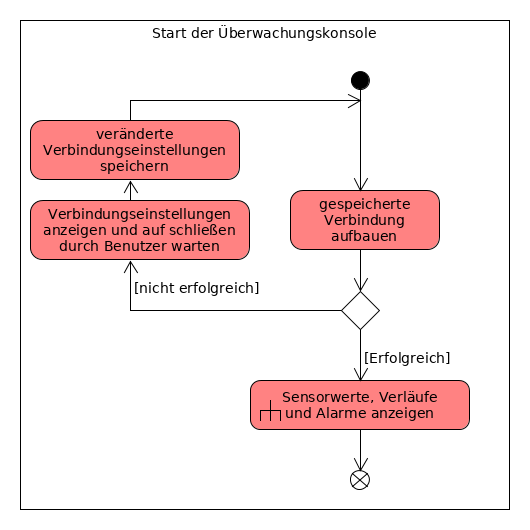
\includegraphics[scale=0.62]{media/Activities/launch-console.png}
  \caption{Aktivitätsdiagram für den Start der Überwachungskonsole}
\end{figure}
\begin{enumerate}[noitemsep]
 \item Die \gls{Uberwachungskonsole} versucht, die Verbindung zu den \glspl{OPC UA Server} mit den zuletzt gespeicherten \glspl{Verbindungsinformation} aufzunehmen.
 \item Wenn der Verbindungsaufbau fehlschlägt, öffnet sich das Fenster mit den Verbindungseinstellungen. Wenn der Benutzer das Fenster wieder schließt,
 werden die veränderten \glspl{Verbindungsinformation} gespeichert und erneut versucht, die Verbindung aufzubauen.
 \item Wenn der Verbindungsaufbau geklappt hat, zeigt die \gls{Uberwachungskonsole} die übertragenen Werte der \gls{Fertigungssimulation}, sowie die
 Alarme und Verläufe an.
 \item Wenn der Benutzer die \gls{Uberwachungskonsole} schließt, ist das Programm beendet.
\end{enumerate}

\subsubsection{Hauptschleife und Alarme der Überwachungskonsole}
\begin{figure}[H]
  \centering
  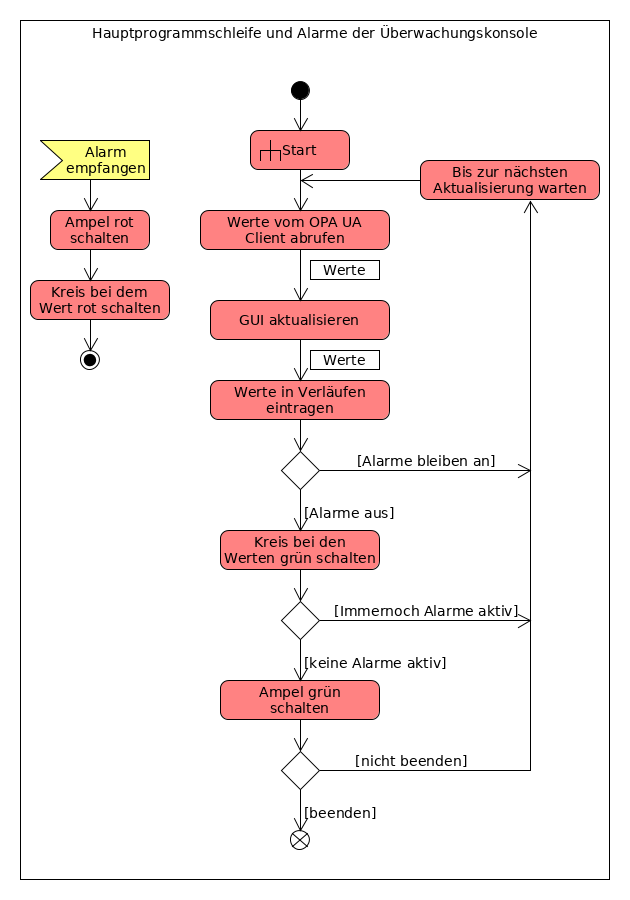
\includegraphics[scale=0.62]{media/Activities/main-console.png}
  \caption{Aktivitätsdiagram für die Hauptschleife und Alarme der Überwachungskonsole}
\end{figure}

\emph{Hauptschleife}
\begin{enumerate}[noitemsep]
 \item Die Überwachungskonsole startet, wie in \ref{console-launch} beschrieben.
 \item Die Überwachungskonsole ruft die aktuellen Sensorwerte vom \gls{OPC UA Server} ab.
 \item Diese Werte werden auf den Anzeigen der \gls{Uberwachungskonsole} angezeigt.
 \item Dann werden diese Werte in den Verlauf (sofern aktiviert) eingefügt.
 \item Wenn bei einem aktivem Alarm die Alarmbedingung nicht mehr erfüllt ist, wird er ausgeschaltet.
 \item Wenn keine Alarme mehr aktiv sind, wird die Ampel auf grün geschaltet.
 \item Wenn der Benutzer das Fenster geschlossen hat, wird die \gls{Uberwachungskonsole} nun beendet.
 \item Vor der nächsten Aktualisierung wird gewartet, damit erst nach der Aktualisierungsfrequenz erneut Sensorwerte abgerufen werden.
\end{enumerate}
\emph{Alarme empfangen}
\begin{enumerate}[noitemsep]
 \item Wenn ein Alarm empfangen wird, wird die Ampel auf rot geschaltet.
 \item Dann wird der Kreis bei den Anzeigen auf rot geschaltet.
\end{enumerate}

\subsubsection{Hauptschleife der Fertigungssimulation}
\begin{figure}[H]
  \centering
  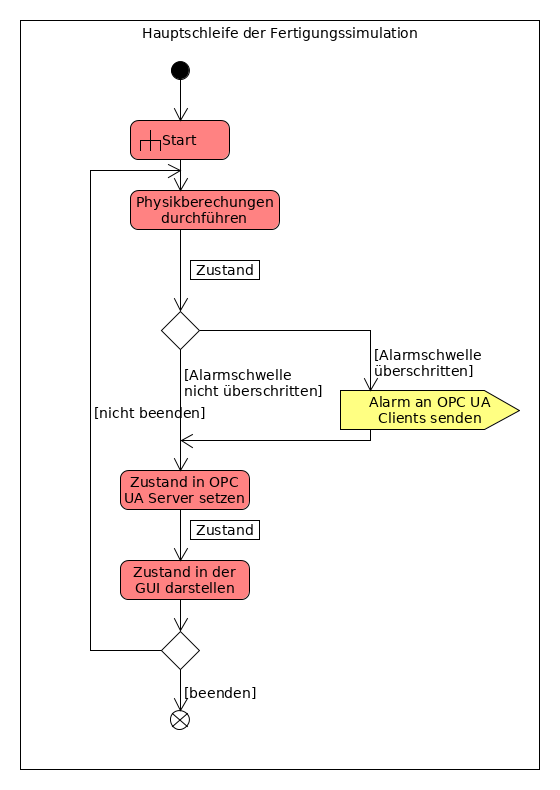
\includegraphics[scale=0.62]{media/Activities/main-simulation.png}
  \caption{Aktivitätsdiagram für die Hauptschleife der Fertigungssimulation}
\end{figure}

\begin{enumerate}[noitemsep]
 \item Die Fertigungssimulation startet.
 \item Der Zustand der \gls{Fertigungssimulation} wird berechnet.
 \item Wenn durch eine Zustandsänderung eine Alarmschwelle überschritten wurde, wird der Alarm an alle \glspl{OPC UA Client} gesendet,
 die sich für den Alarm registriert haben.
 \item Danach wird der geänderte Zustand im \gls{OPC UA Server} gesetzt.
 \item Dann wird der aktualisierte Zustand in der \gls{GUI} angezeigt.
 \item Wenn der Benutzer das Fenster geschlossen hat, wird die \gls{Fertigungssimulation} nun beendet.
\end{enumerate}

\subsection{Statische Modelle}
\subsubsection{Komponentendiagramm}
\begin{figure}[H]
  \centering
  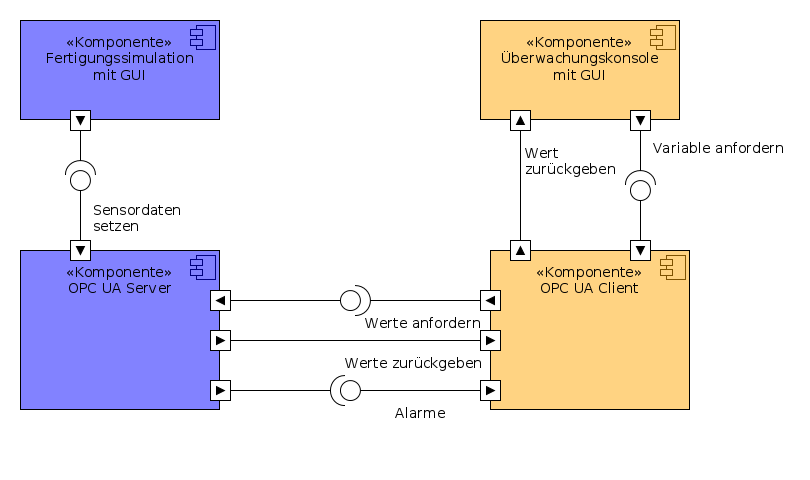
\includegraphics[scale=0.5]{media/ComponentDiagram/componentDiagram.png}
  \caption{Komponentendiagramm}
\end{figure}

Die \gls{Fertigungssimulation} simuliert die Werte f\"ur die Tanks. Sie zeigt in ihrer \gls{GUI} eine schematische Darstellung der
\gls{Produktionsanlage}. Die \gls{Produktionsanlage} l\"asst sich \"uber die \gls{Fertigungssimulation} steuern. Die \gls{Fertigungssimulation} setzt
in den \glslink{OPC UA Server}{OPC UA Servern} die "`gemessenen"' Werte.

Die \glspl{OPC UA Server} aggregieren mehrere \glspl{Sensordatum}, die durch die \gls{Fertigungssimulation} gesetzt werden. An jedem \gls{OPC UA Server} k\"onnen
sich 0 bis beliebig viele \glspl{OPC UA Client} registrieren. Auf Anfrage erhalten die \glspl{OPC UA Client} \glspl{Sensordatum}. Bei einem \gls{OPC UA Server} registrierte
Alarme werden an die \glspl{OPC UA Client} geschickt wo n\"otig.

Die \glspl{OPC UA Client} sind bei je genau einem \gls{OPC UA Server} registriert. Sie fragen, wenn sie von der \gls{Uberwachungskonsole} dazu
aufgefordert werden, die Daten von ihrem jeweiligen \gls{OPC UA Server} ab. Sie k\"onnen bei ihrem \gls{OPC UA Server} Alarme registrieren und diese
dann empfangen. Die \glspl{OPC UA Client} stellen der \gls{Uberwachungskonsole} Daten bereit.

Die \gls{Uberwachungskonsole} verwendet mehrere \glspl{OPC UA Client}, um \"uber diese und die \glspl{OPC UA Server} Daten von der
\gls{Fertigungssimulation} zu erhalten. \"Uber sie werden die \glspl{OPC UA Client} indirekt gesteuert. In der \gls{Uberwachungskonsole} kann der Benutzer Alarme
f\"ur die \glspl{OPC UA Client} registrieren und angeben, welche Daten von den \glslink{OPC UA Server}{OPC UA Servern} abgefragt werden sollen. Die Daten und Alarme, die
die \gls{Uberwachungskonsole} von den \glspl{OPC UA Client} erh\"alt, stellt sie graphisch dar.

Die einzige Verbindung von \gls{Uberwachungskonsole} und \gls{Fertigungssimulation} ist \"uber die \glspl{OPC UA Server} und \glspl{OPC UA Client} realisiert.

\section{Nutzerinterface-Skizzen}
\subsection{Fertigungssimulation}
\begin{figure}[H]
  \centering
  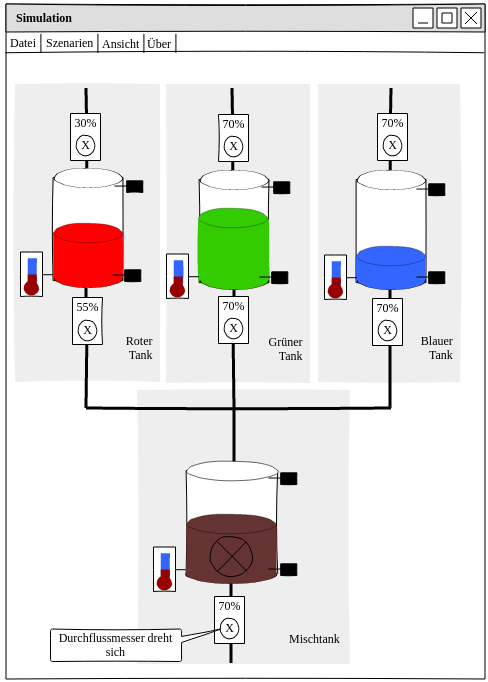
\includegraphics[scale=0.5]{media/ui-server/ui-server-main.png}
  \caption{Nutzerinterface-Skizze des Hauptfensers der Fertigungssimulation}
\end{figure}
Im Hauptfenster der \gls{Fertigungssimulation} wird die simulierte \gls{Produktionsanlage} angezeigt. Dabei wird jeder der Tanks
mit einem blassgrauen Kasten hinterlegt, um den Zuständigkeitsbereich der einzelnen \gls{OPC UA Server} abzugrenzen. Die Anzeige wird
in Echtzeit von der Simulation aktualisiert. Die Anzeigen der Durchflussmesser, sowie der Motor im unteren Tank drehen sich.
Die Tanks werden als Zylinder dargestellt, die in der entsprechenden Farbe gefüllt sind.

\begin{figure}[H]
  \centering
  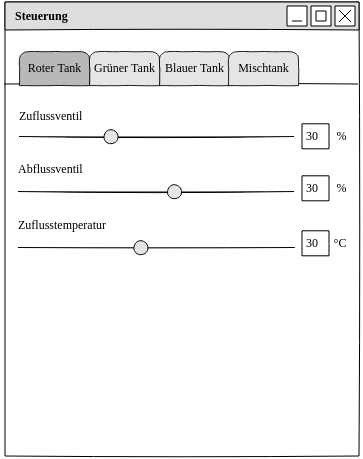
\includegraphics[scale=0.5]{media/ui-server/ui-server-control.png}
  \caption{Nutzerinterface-Skizze des Steuerungsfensters der Fertigungssimulation}
\end{figure}
Über das Menü kann ein Fenster angezeigt werden, das die Konfiguration der einzelnen \glspl{Prozessvariable} erlaubt. Hierbei
wird für den Zuständigkeitsbereich jedes \glslink{OPC UA Server}{OPC UA Servers} ein Reiter angezeigt. Die Reiter beziehen sich also
direkt auf die dargestellten blassgrauen Kästen. Die Einstellunge der jeweiligen \glspl{Prozessvariable} erfolgt über Schieberegler.

\begin{figure}[H]
  \centering
  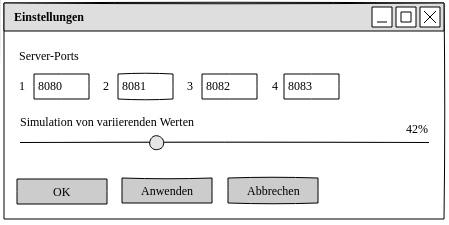
\includegraphics[scale=0.5]{media/ui-server/ui-server-settings.png}
  \caption{Nutzerinterface-Skizze des Einstellungsfensters der Fertigungssimulation}
\end{figure}
Im Einstellungsdialog können die Ports der jeweiligen Server über Textfelder eingestellt werden. Der Jitter kann über einen Schieberegler
eingestellt werden. Es existieren die Buttons "`Abbrechen"', "`Anwenden"' und "`OK"'. 

\pagebreak

\subsection{Überwachungskonsole}
\begin{figure}[H]
  \centering
  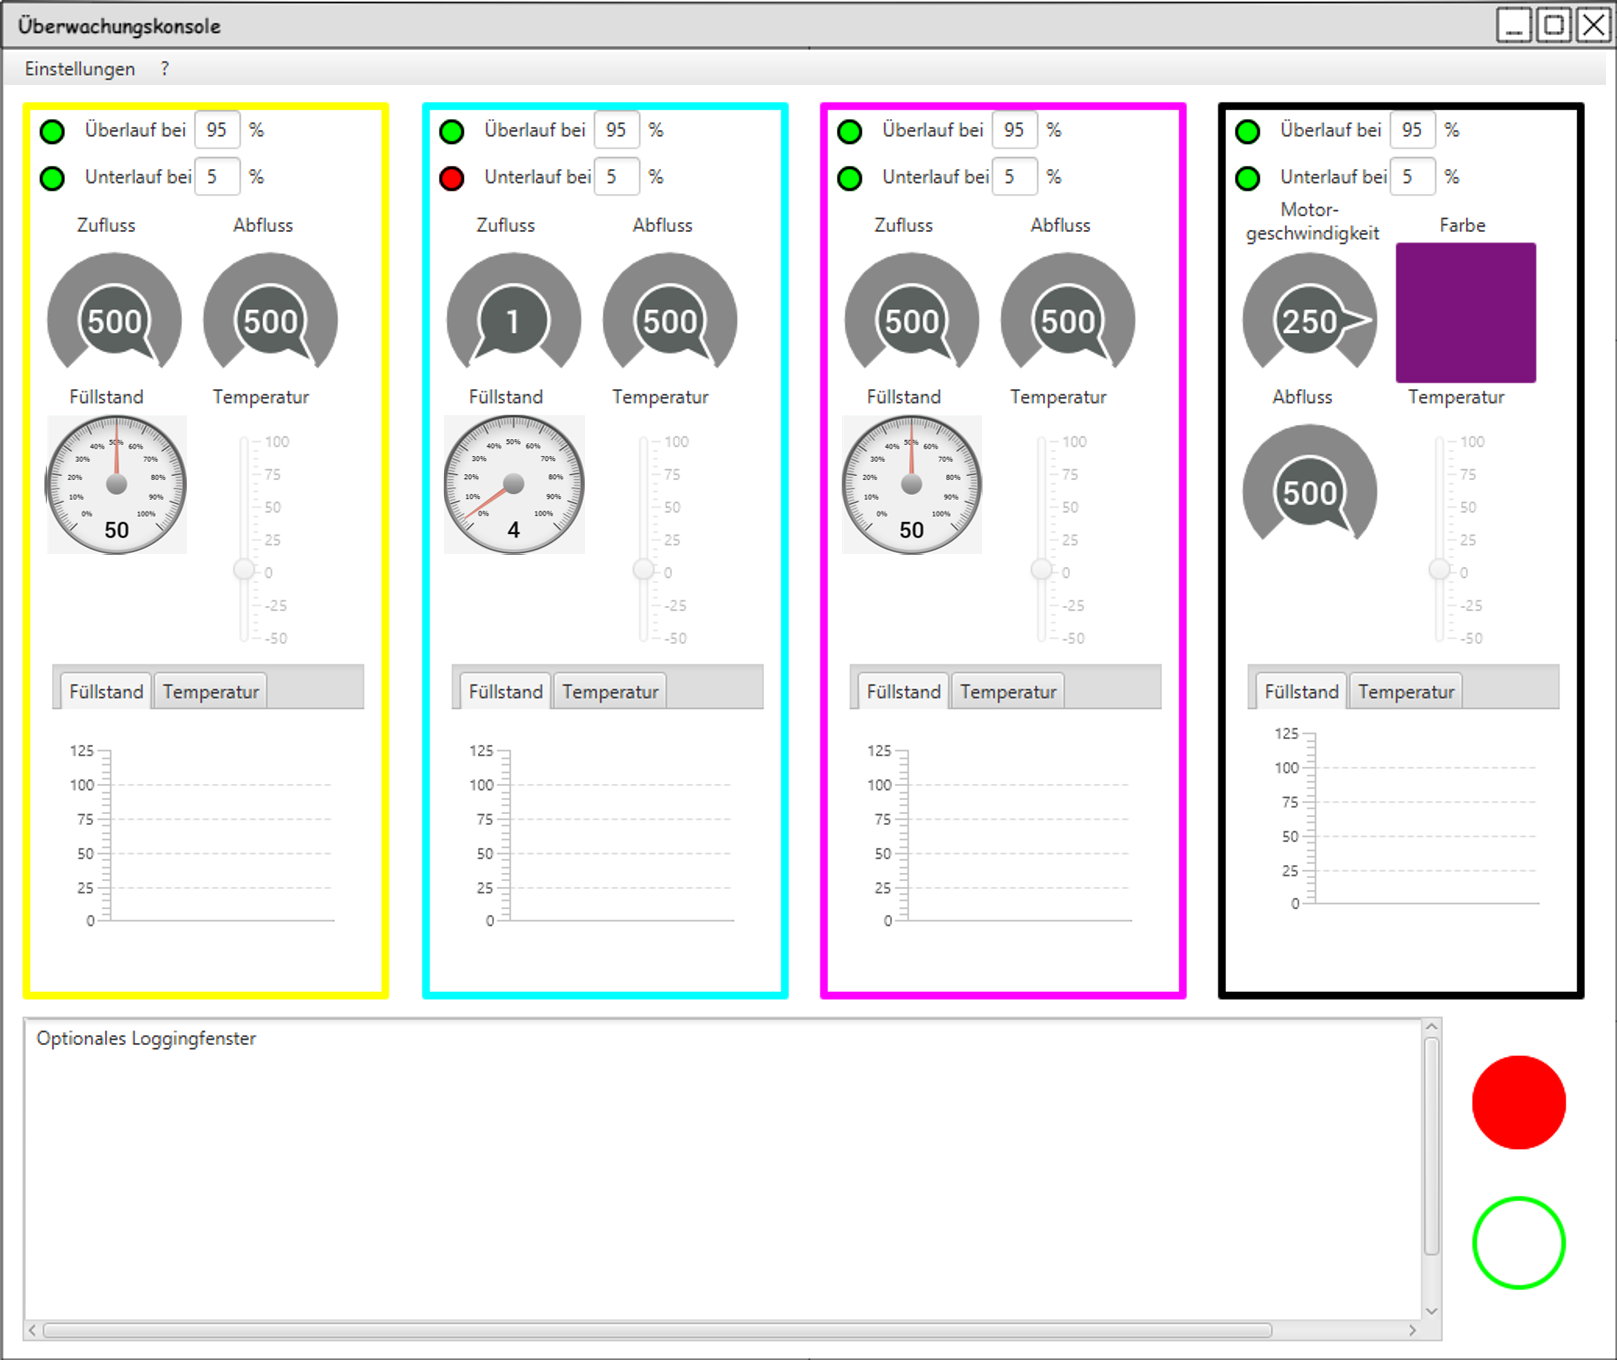
\includegraphics[scale=0.5]{media/ui-client/ui-uw.png}
  \caption{Nutzerinterface-Skizze des Hauptfensters der Überwachungskonsole}
\end{figure}
Im Hauptfenster der \gls{Uberwachungskonsole} werden die Anzeigen für die \glspl{Sensordatum} für jeden Tank in einem einzelnen Rahmen gesammelt. Dabei repräsentieren die Anzeigen im roten, grünen bzw. blauen Rahmen den roten, grünen bzw. blauen Tank. Die Anzeigen im schwarzen Rahmen repräsentieren den Mischtank, dessen Farbe explizit angezeigt wird.
Neben den Anzeigen der \glspl{Sensordatum} sind auch die Füllstands- und Temperaturverläufe in Form von Graphen und die Alarme enthalten. Im grünen Tank ist beispielhaft der Alarm für einen Unterlauf ausgelöst.
Darüber hinaus enthält das Hauptfenster das Loggingfenster und die Ampel für den allgemeinen Zustand der \gls{Uberwachungskonsole}.

\begin{figure}[H]
	\centering
	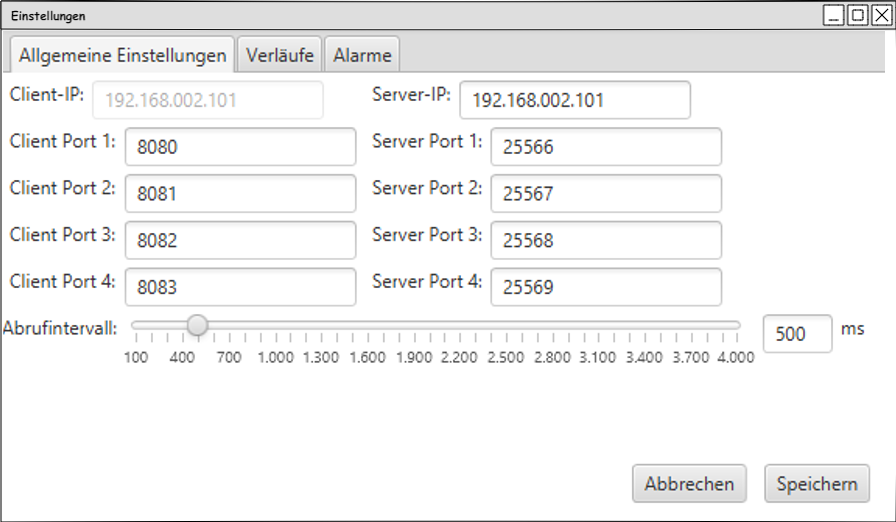
\includegraphics[scale=0.5]{media/ui-client/ui-uw-settings1.png}
	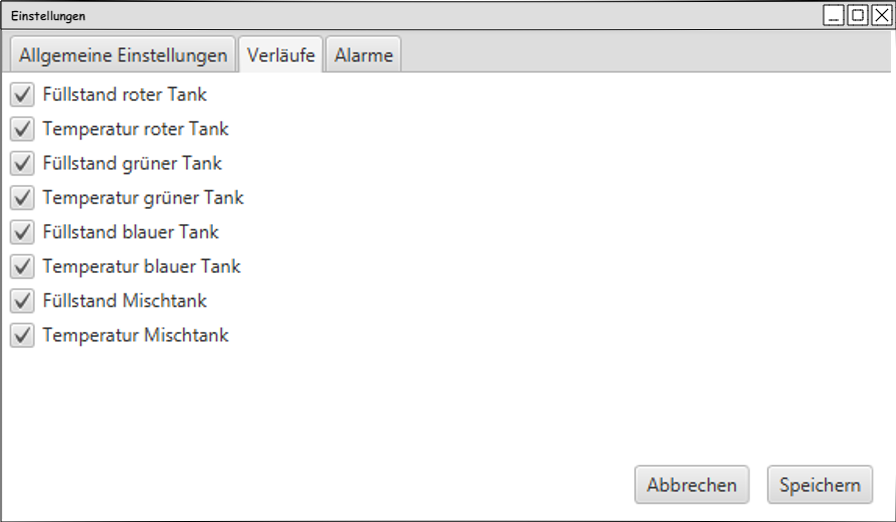
\includegraphics[scale=0.5]{media/ui-client/ui-uw-settings2.png}
	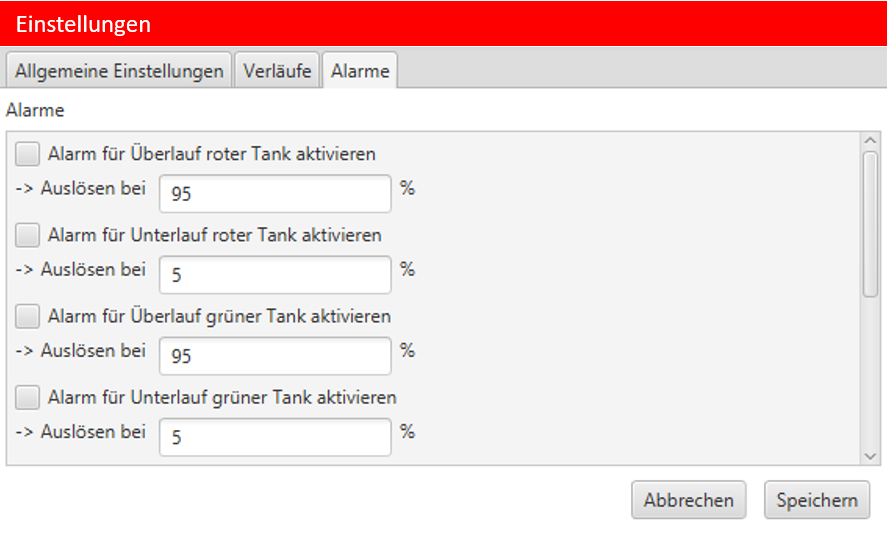
\includegraphics[scale=0.5]{media/ui-client/ui-uw-settings3.png}
	\caption{Nutzerinterface-Skizze des Einstellungsdialogs der Überwachungskonsole}
\end{figure}
Im Einstellungsdialog sind bereits alle möglichen Einstellungen skizziert. Dem entsprechend beinhalten die "Allgemeinen Einstellungen" die \glspl{Verbindungsinformation}, die Sprache und die Aktualisierungsfrequenz, die "Verläufe" das Ein- und Ausschalten der einzelnen Füllstands- und Temperaturverläufe und die "Alarme" das Einstellen dieser.

\begin{figure}[H]
	\centering
	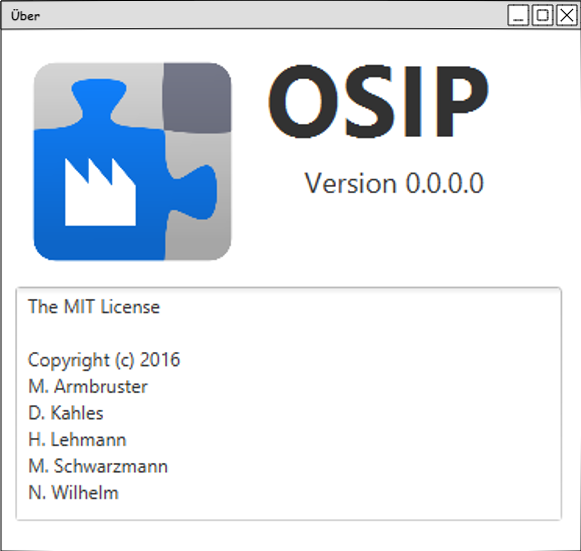
\includegraphics[scale=0.5]{media/ui-client/ui-uw-uber.png}
	\caption{Nutzerinterface-Skizze des "`Über"'-Fensters der Überwachungskonsole}
\end{figure}
Das "`Über"'-Fenster der \gls{Uberwachungskonsole} enthält die Programm- und Lizenzinformationen zum Projekt. Daneben bietet es im Lizenztextfeld Platz für die Lizenzen verwendeter Projekte; es kann aber auch um ein separates Feld für diese Lizenzen erweitert werden.

\pagebreak
\printglossaries

\pagebreak
\phantomsection
\addcontentsline{toc}{section}{\listfigurename}
\listoffigures

\end{document}
